% =====================================================
% Part C: The Blueprint - System Architecture and Design (30%)
% =====================================================

\section{System Architecture and Design}

HorizonBench is designed to simulate the complete peer review pipeline of top-tier academic conferences. Unlike existing systems that collapse review into single-pass generation, our architecture models the full workflow: from paper understanding through dynamic benchmark construction, multi-dimensional evaluation, to multi-model consensus with meta-review synthesis. This section details the four-phase architecture illustrated in Figure~\ref{fig:system_overview}.

\begin{figure}[t]
    \centering
    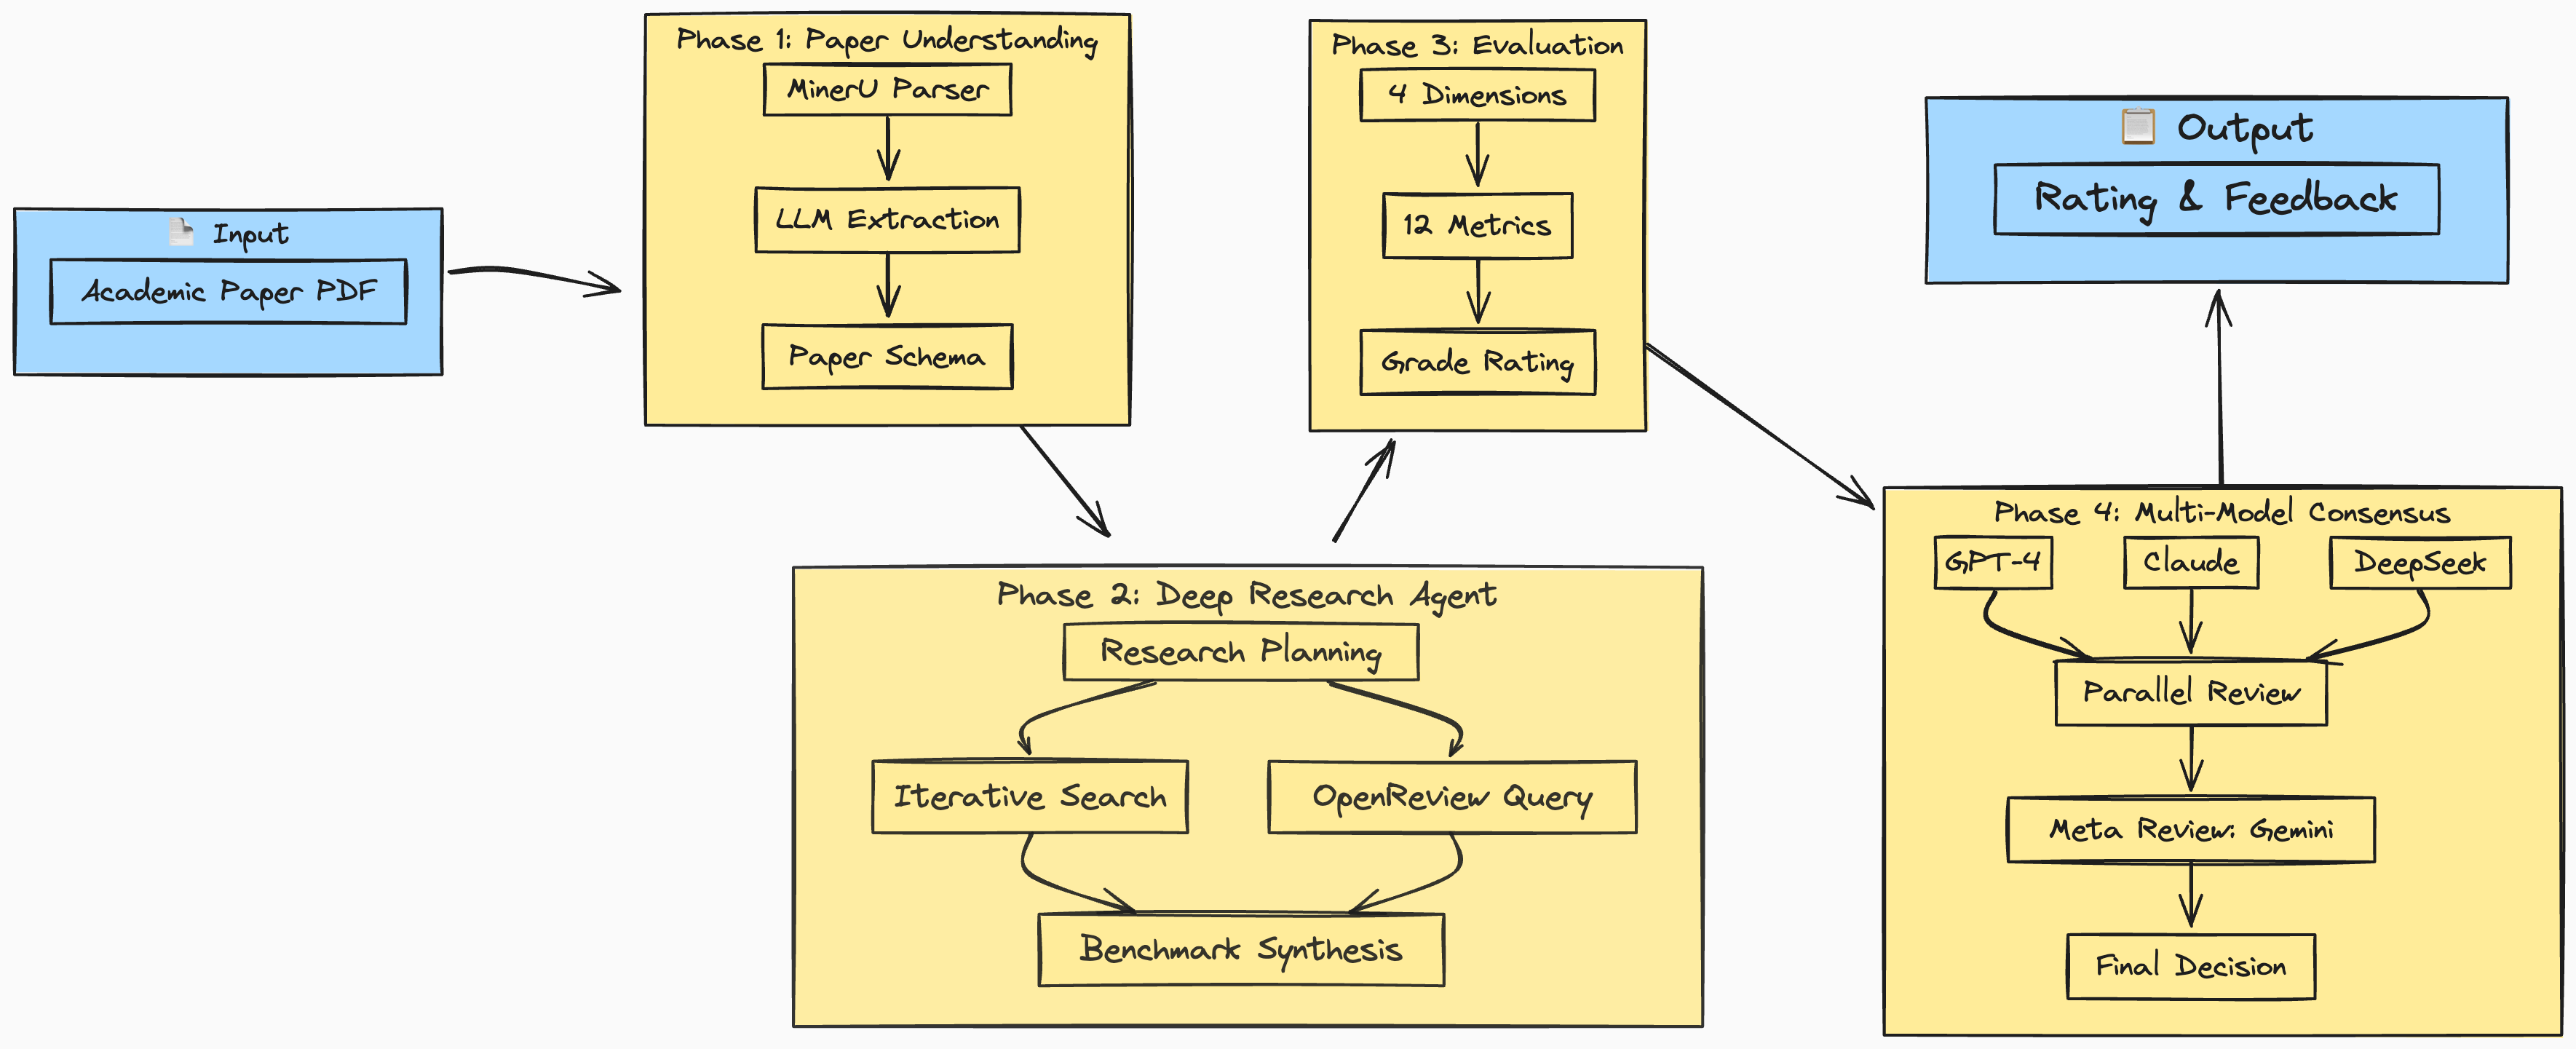
\includegraphics[width=\linewidth]{figures/system_overview.png}
    \caption{HorizonBench System Overview. The four-phase pipeline transforms raw PDF input into comprehensive evaluation reports through paper understanding, dynamic benchmark construction, multi-dimensional assessment, and multi-model consensus.}
    \label{fig:system_overview}
\end{figure}

% -------------------------------------------------
\subsection{Overall Architecture}
% -------------------------------------------------

Table~\ref{tab:phase_overview} summarizes the four phases of HorizonBench, mapping each to its corresponding real-world peer review component.

\begin{table}[h]
\centering
\caption{Four-Phase Architecture Overview}
\label{tab:phase_overview}
\small
\begin{tabular}{@{}llll@{}}
\toprule
\textbf{Phase} & \textbf{Name} & \textbf{Core Task} & \textbf{Output} \\
\midrule
1 & Paper Understanding & PDF parsing, content extraction & Paper Schema \\
2 & Deep Research Agent & Dynamic benchmark construction & Contextualized Benchmark \\
3 & Multi-Dimensional Evaluation & 4 dimensions, 12 fine-grained metrics & Dimension Ratings \\
4 & Multi-Model Consensus & 3 reviewers + meta-review & Final Report \\
\bottomrule
\end{tabular}
\end{table}

The design philosophy mirrors actual conference review processes: Phase 1 corresponds to a reviewer reading the paper; Phase 2 represents the reviewer's domain expertise and literature awareness; Phase 3 maps to structured evaluation against review criteria; and Phase 4 simulates the Area Chair synthesizing multiple reviewer opinions into a final decision.

% -------------------------------------------------
\subsection{Data Pipeline}
% -------------------------------------------------

\subsubsection{Data Source}

The primary data source is the ACL Anthology\footnote{\url{https://aclanthology.org}}, providing academic papers from ACL conferences and workshops. For dynamic benchmark construction, we integrate three external sources: Semantic Scholar API for comprehensive literature search, arXiv for preprints, and OpenReview for real peer review data including both accepted and rejected submissions.

\subsubsection{Data Requirements}

HorizonBench adopts a few-shot prompting approach, eliminating the need for large-scale training data. Instead, we require: (1) \textbf{Input data}: Raw PDF files from the ACL corpus; (2) \textbf{Few-shot examples}: Real peer reviews from OpenReview spanning Strong Accept to Strong Reject; (3) \textbf{Evaluation data}: A gold-standard subset with expert annotations for system validation, utilizing the PeerRead dataset~\cite{kang2018peerread} containing 14.7K papers with 10.7K expert reviews.

\subsubsection{Phase 1: Paper Understanding}

Phase 1 transforms unstructured PDF documents into structured, machine-readable representations. Figure~\ref{fig:paper_understanding} illustrates this pipeline.

\begin{figure}[t]
    \centering
    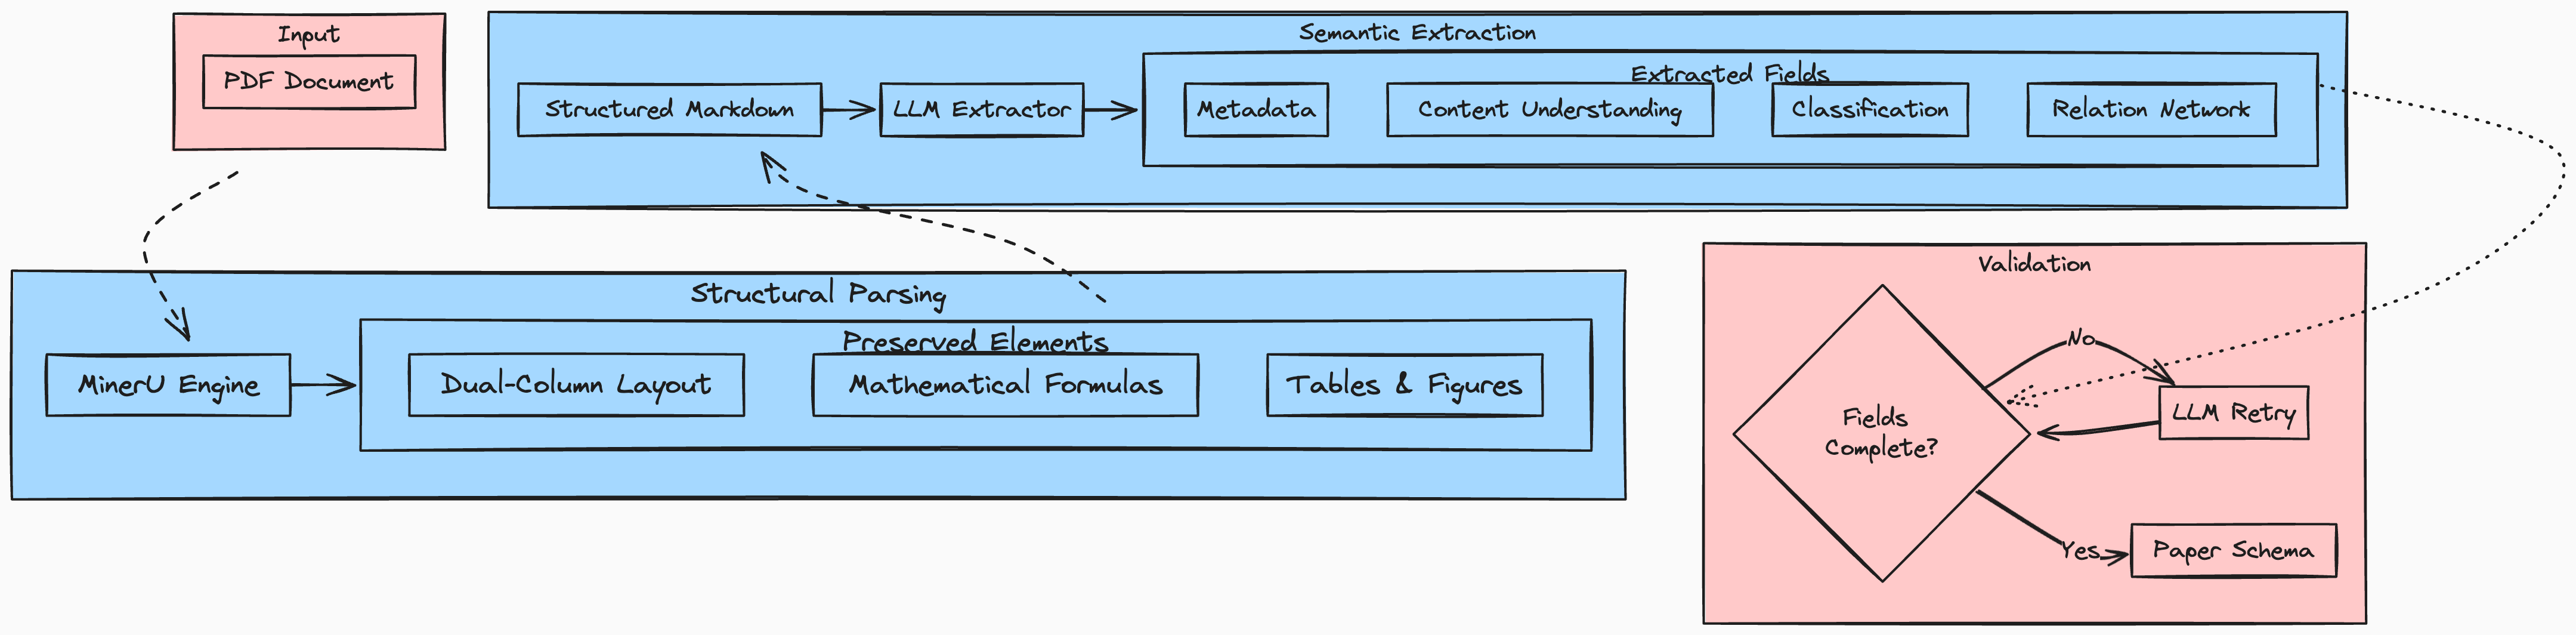
\includegraphics[width=\linewidth]{figures/paper_understanding.png}
    \caption{Phase 1: Paper Understanding Pipeline. MinerU handles structural parsing while LLM performs semantic extraction, producing a comprehensive Paper Schema.}
    \label{fig:paper_understanding}
\end{figure}

\paragraph{Technical Selection.} We employ MinerU (Magic-PDF)~\cite{mineru2024} for PDF parsing, selected for its superior handling of academic document structures including dual-column layouts, mathematical formulas, and complex tables. Unlike vision-based OCR approaches that may lose semantic structure, MinerU preserves hierarchical organization through layout-aware parsing.

\paragraph{Processing Pipeline.} The workflow proceeds as: PDF $\rightarrow$ MinerU Parsing $\rightarrow$ Structured Markdown $\rightarrow$ LLM Content Extraction $\rightarrow$ Field Validation $\rightarrow$ Paper Schema. The LLM extraction step employs GPT-4 or Claude to identify semantic elements that rule-based parsing cannot capture, such as implicit research contributions or methodology innovations.

\paragraph{Output Schema.} The Paper Schema contains four components: (1) \texttt{paper\_metadata}: title, authors, venue, year; (2) \texttt{content\_understanding}: abstract, research problem, methodology, contributions, conclusions, limitations; (3) \texttt{classification}: domain, sub-domain, paper type, keywords; (4) \texttt{relation\_network}: compared baselines, used datasets, and seminal references. The \texttt{relation\_network} specifically supports Phase 2's ``snowball'' literature discovery by extracting not just content but relational context.

% -------------------------------------------------
\subsection{Core Models}
% -------------------------------------------------

\subsubsection{Phase 2: Deep Research Agent}

A critical limitation of existing review systems is static evaluation against fixed criteria without domain-specific context. HorizonBench addresses this through a Deep Research Agent that dynamically constructs benchmarks for each paper. Figure~\ref{fig:deep_research} illustrates this agentic workflow.

\begin{figure}[t]
    \centering
    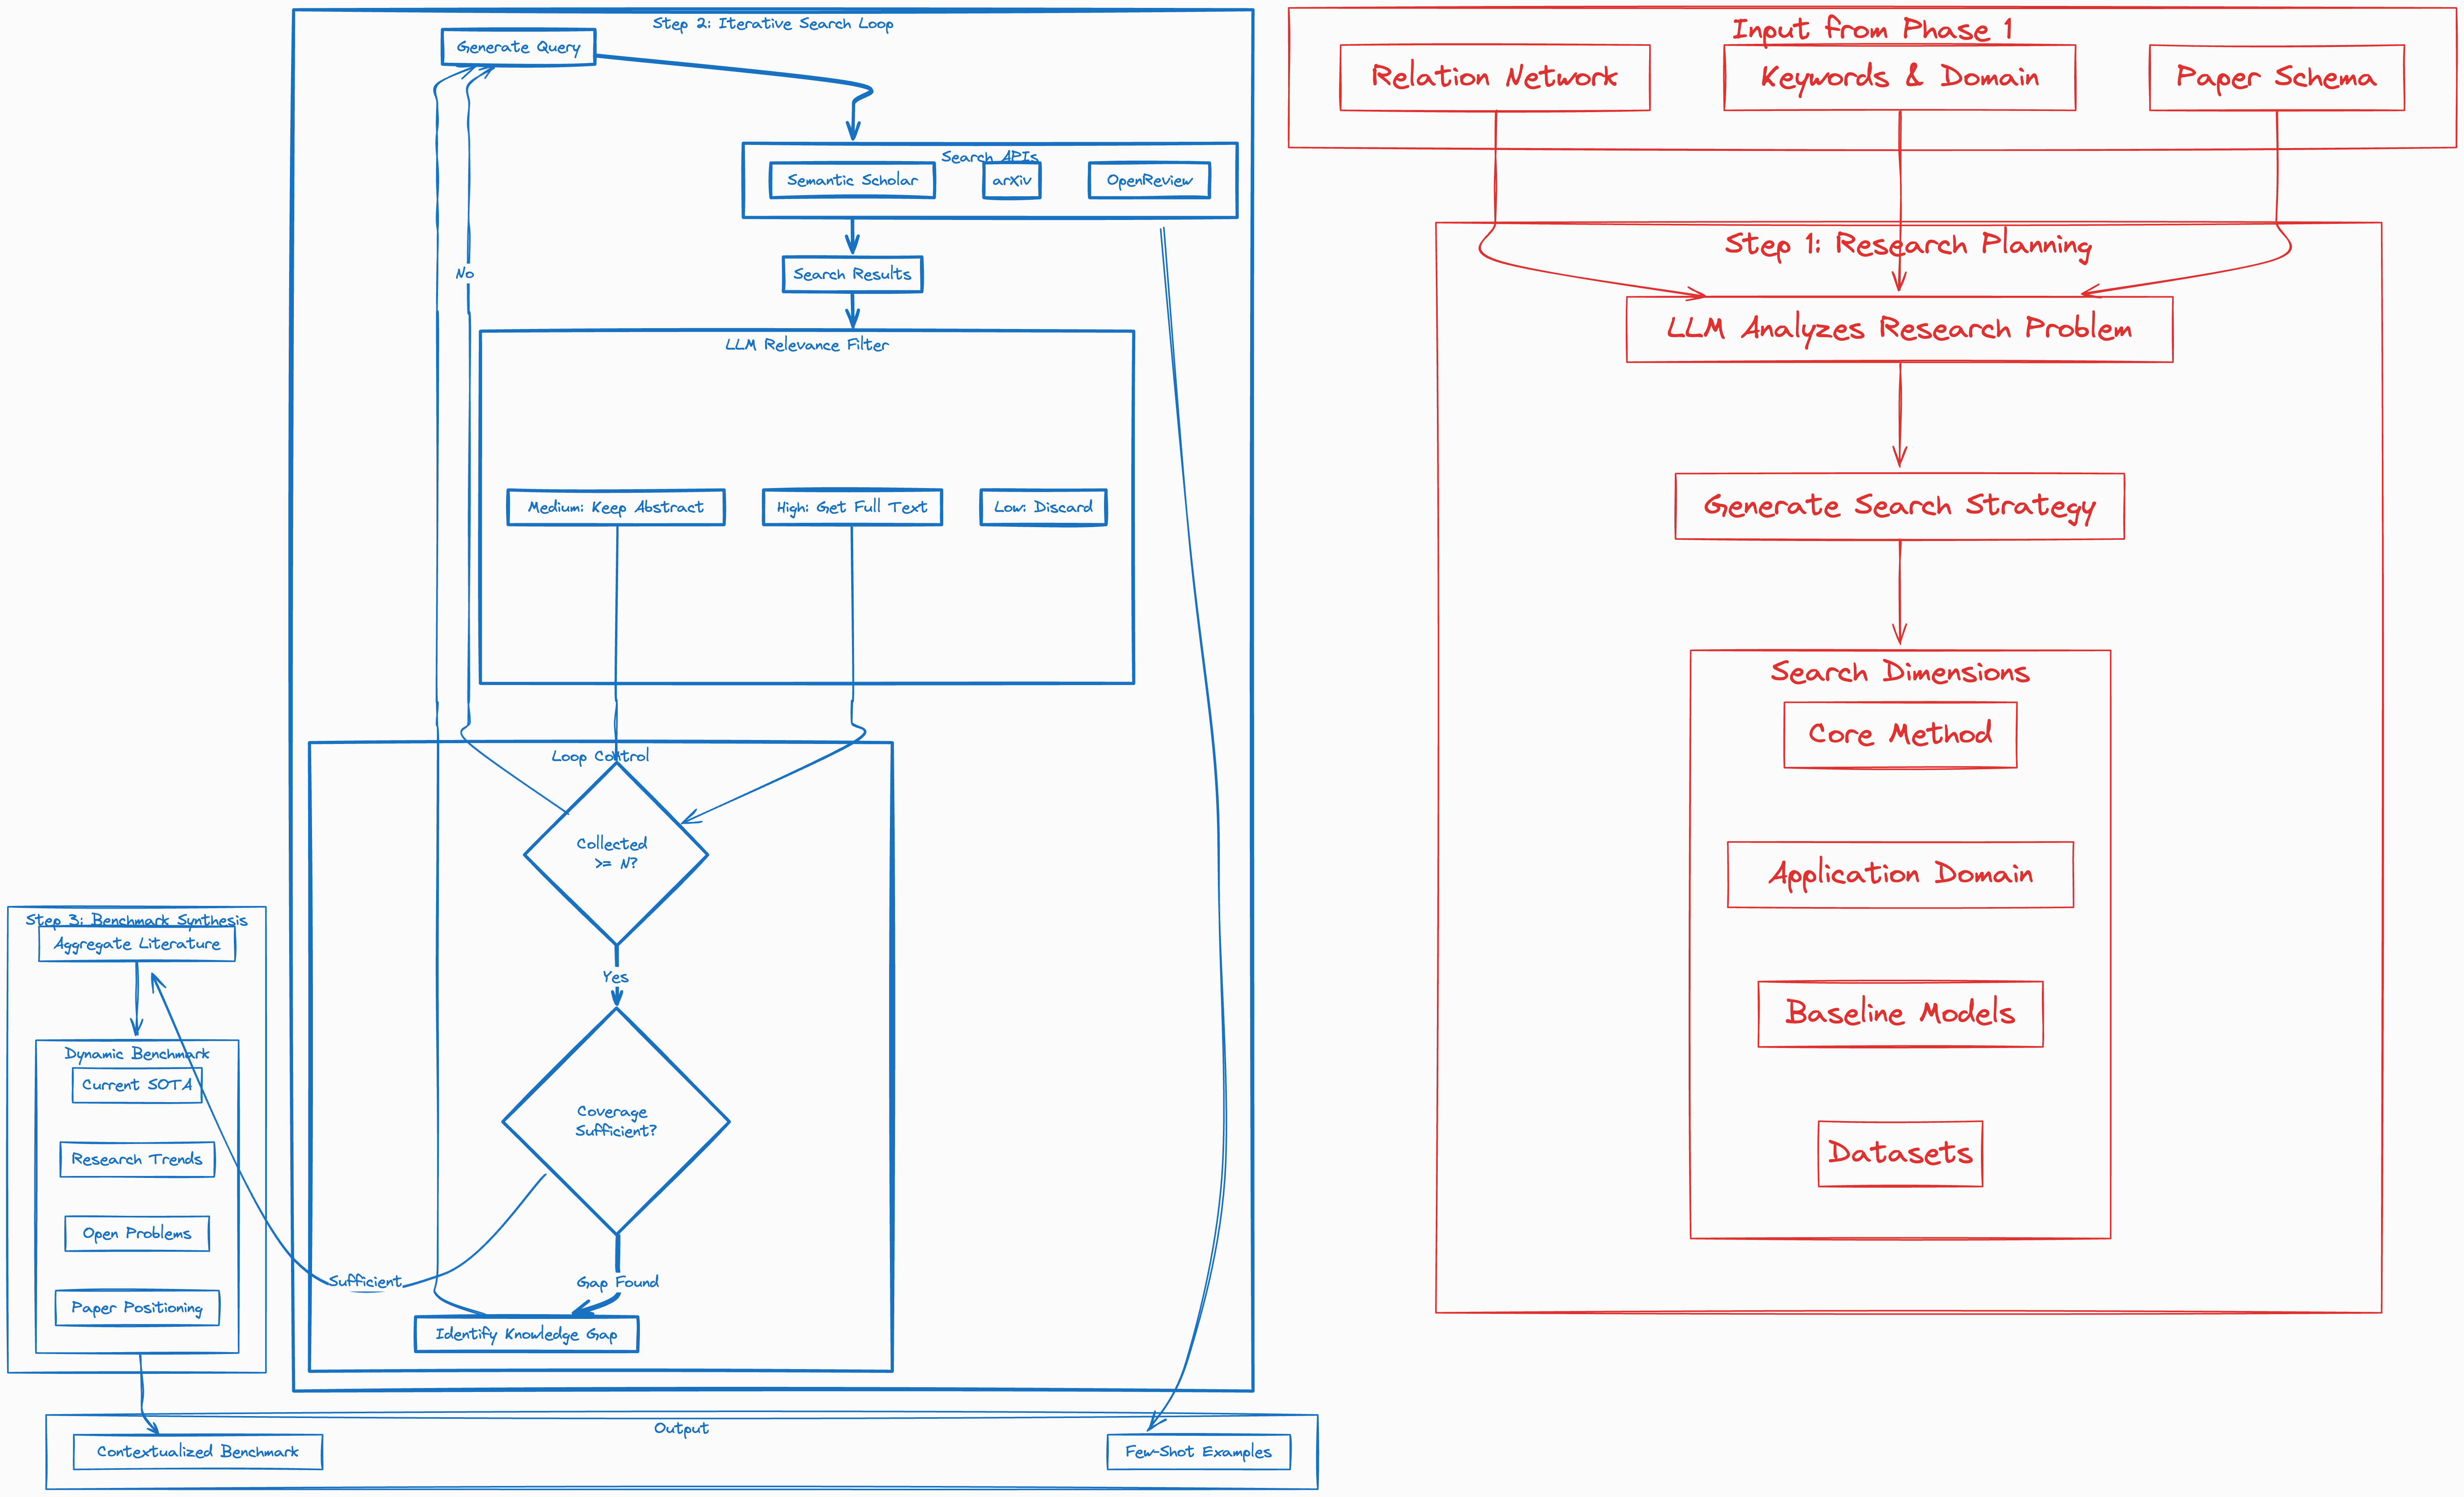
\includegraphics[width=\linewidth]{figures/deep_research.png}
    \caption{Phase 2: Deep Research Agent. The agent autonomously plans search strategies, iteratively retrieves literature, and synthesizes a contextualized benchmark report.}
    \label{fig:deep_research}
\end{figure}

\paragraph{Agentic Design Philosophy.} Inspired by recent advances in research agents~\cite{zheng2025deepresearch}, we delegate key decisions to the LLM rather than using fixed rules:

\begin{itemize}[nosep,leftmargin=*]
    \item \textbf{Query Generation}: LLM dynamically generates multi-round search queries based on evolving understanding
    \item \textbf{Termination Condition}: LLM judges when coverage is sufficient rather than fixed top-K retrieval
    \item \textbf{Relevance Assessment}: LLM determines document relevance and decides retrieval depth (abstract vs. full-text)
\end{itemize}

\paragraph{Search Infrastructure.} The agent queries three APIs: Semantic Scholar (primary, for comprehensive academic search), arXiv (supplementary, for recent preprints), and OpenReview (for real review examples). For highly relevant papers, full-text retrieval is triggered; otherwise, abstracts suffice.

\paragraph{OpenReview Integration.} OpenReview provides unique value through access to: reviewer comments, numerical ratings, author rebuttals, and crucially, \textit{rejected submissions}. This rejection data helps calibrate assessment boundaries---systems trained only on accepted papers lack understanding of the acceptance threshold.

\paragraph{Benchmark Synthesis.} The agent aggregates retrieved literature into a Dynamic Benchmark Report containing: current SOTA methods, research trends, unsolved problems, and the target paper's positioning relative to prior work. This contextualizes subsequent evaluation.

\paragraph{Sparse Results as Signal.} When the agent finds limited related literature despite extensive search, this signals a potentially novel contribution in an emerging or interdisciplinary area. Rather than penalizing such papers, HorizonBench flags this as a positive indicator for the Novelty dimension.

\subsubsection{Phase 4: Multi-Model Consensus}

Single-model evaluation inherits model-specific biases and produces inconsistent outputs across runs. HorizonBench implements heterogeneous multi-model consensus, illustrated in Figure~\ref{fig:multi_model}.

\begin{figure}[t]
    \centering
    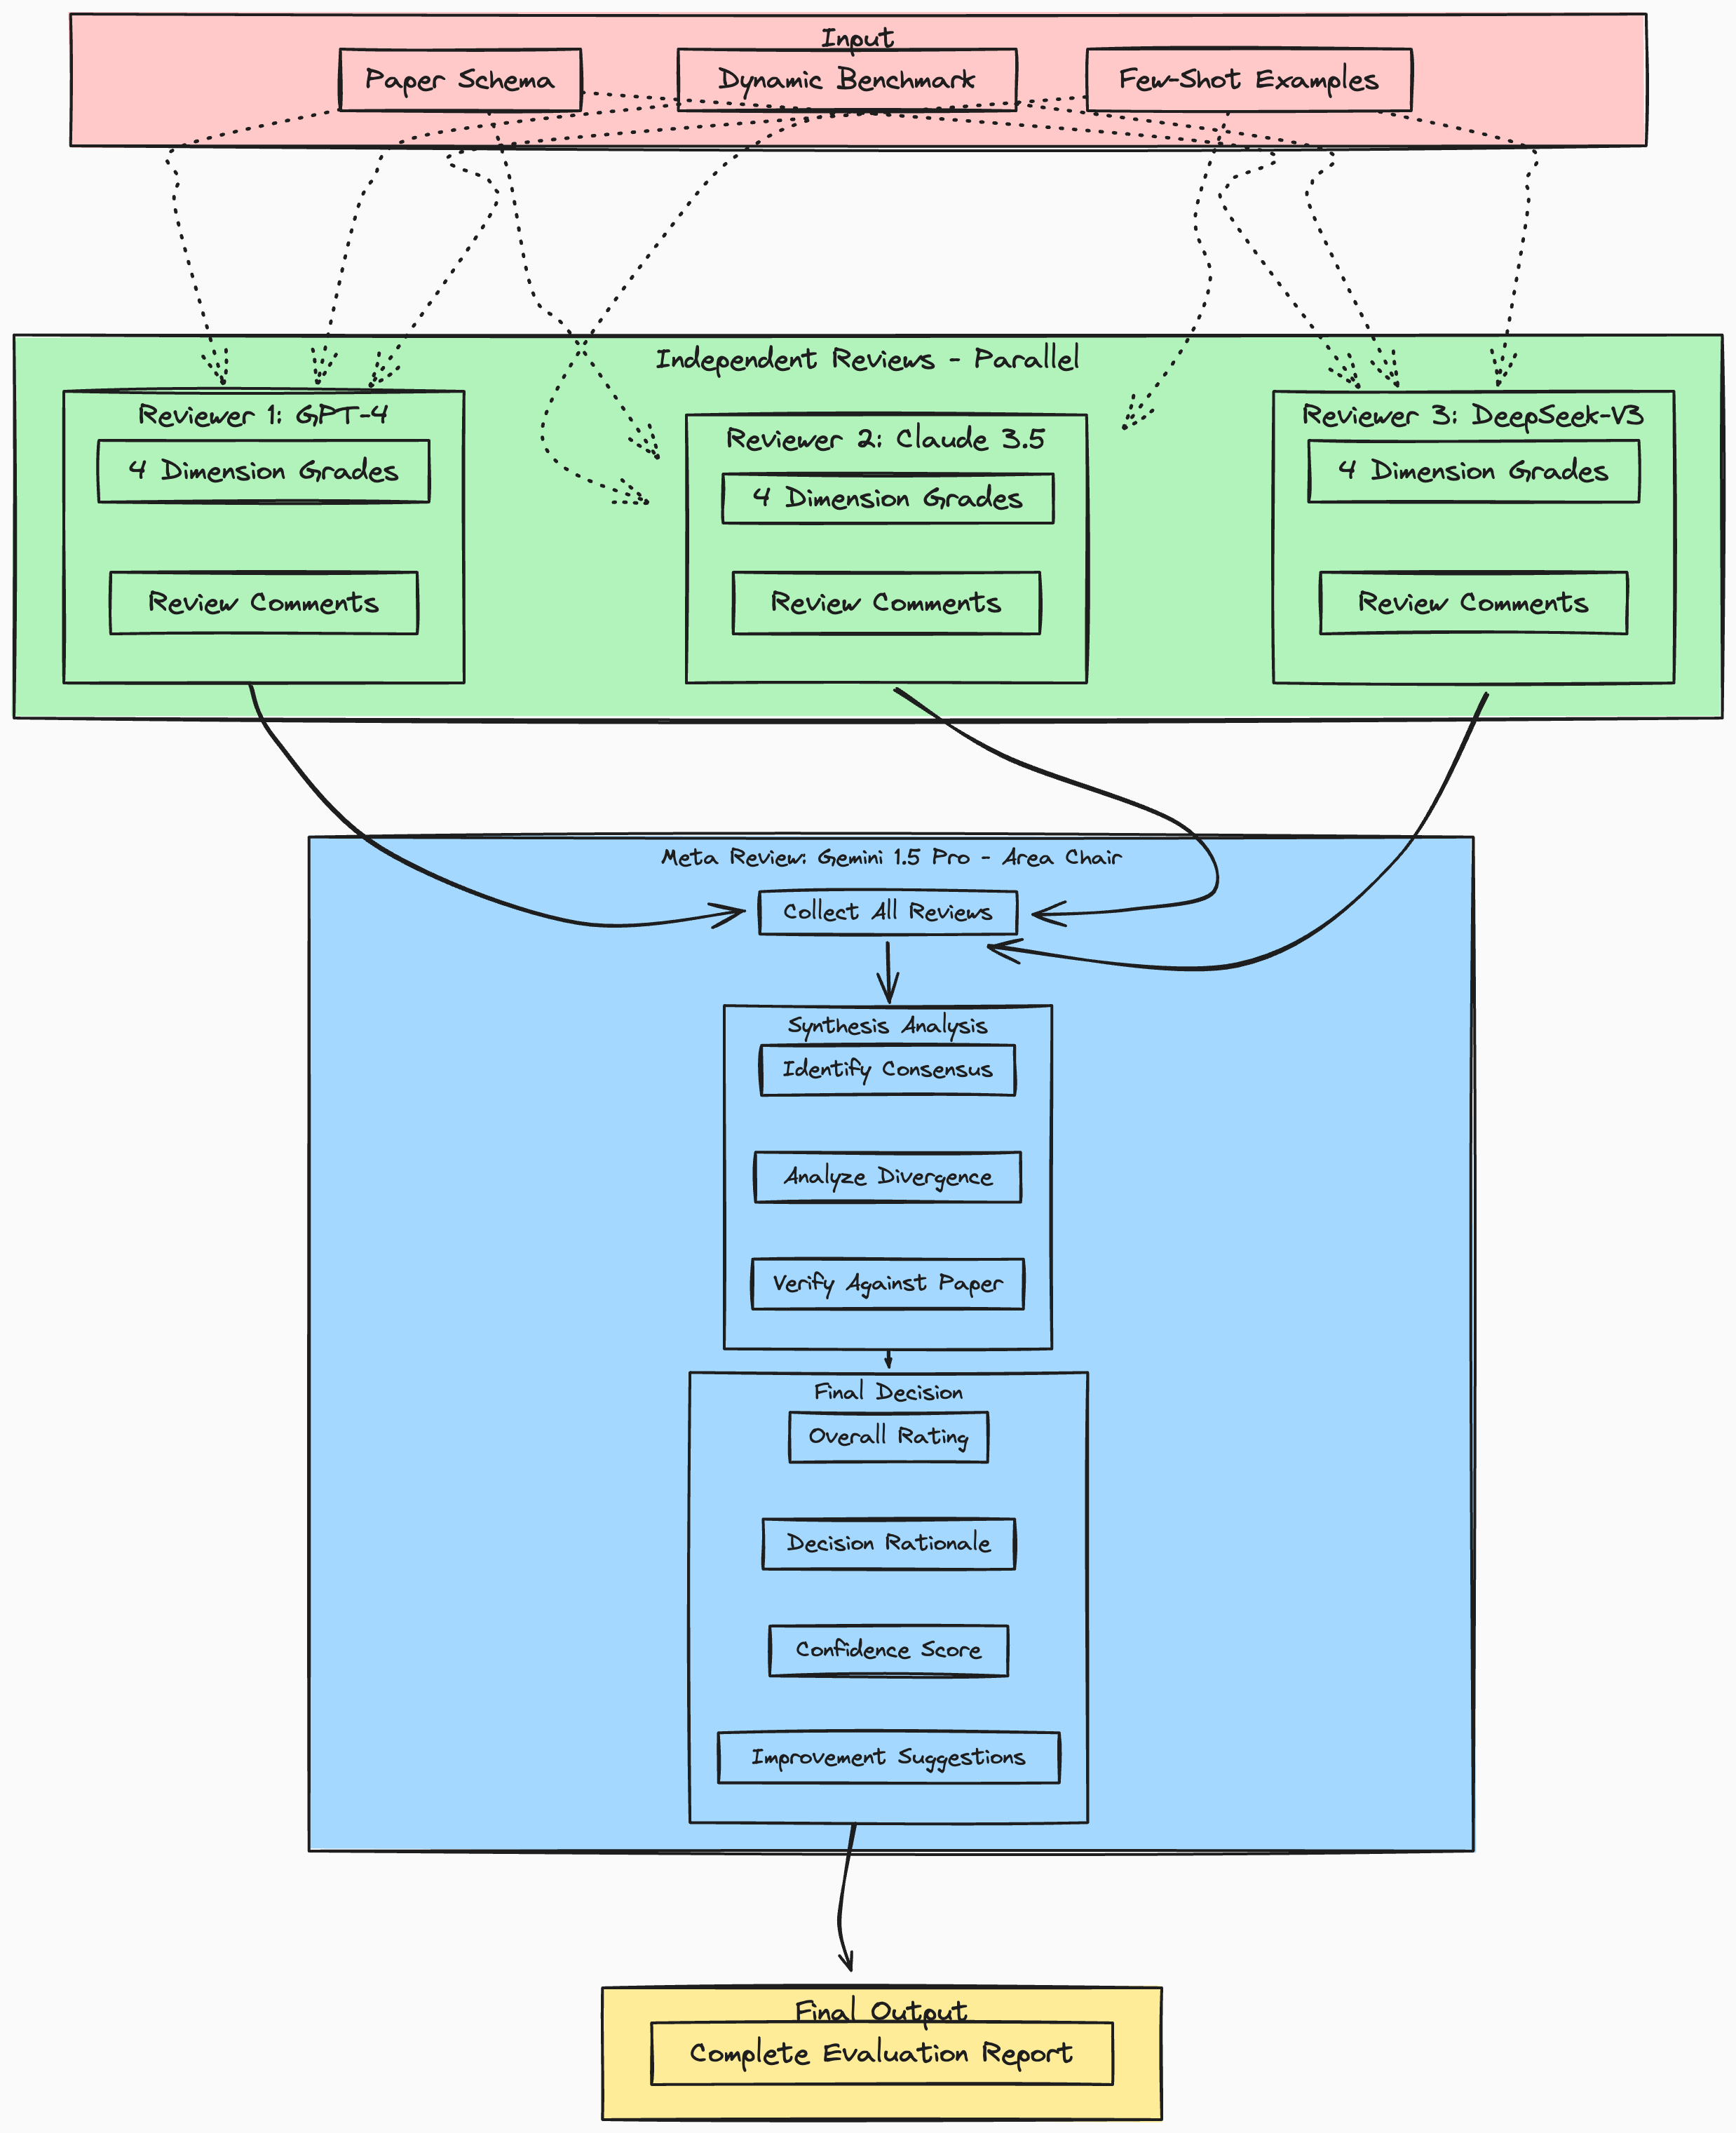
\includegraphics[width=\linewidth]{figures/multi_model.png}
    \caption{Phase 4: Multi-Model Consensus Mechanism. Three independent reviewers (GPT, Claude, DeepSeek) provide parallel assessments, synthesized by a fourth model (Gemini) serving as Area Chair.}
    \label{fig:multi_model}
\end{figure}

\paragraph{Model Selection and Roles.} We employ four distinct model families to maximize diversity:

\begin{itemize}[nosep,leftmargin=*]
    \item \textbf{Reviewer 1}: GPT-4 (OpenAI) --- strong reasoning capabilities
    \item \textbf{Reviewer 2}: Claude 3.5 (Anthropic) --- nuanced analysis
    \item \textbf{Reviewer 3}: DeepSeek-V3 (DeepSeek) --- cost-effective with strong academic text understanding
    \item \textbf{Meta Reviewer}: Gemini 1.5 Pro (Google) --- independent synthesis avoiding self-evaluation bias
\end{itemize}

The critical design choice is using a \textit{fourth} model family for meta-review, ensuring the synthesizer has no stake in any individual review.

\paragraph{Parallel Evaluation Strategy.} All three reviewers receive identical inputs: the Paper Schema, Dynamic Benchmark, and few-shot examples. Each independently produces dimension ratings and textual feedback. This parallel design prevents anchoring effects where early reviews influence later ones.

\paragraph{Meta-Review Mechanism.} The Gemini-based Meta Reviewer performs four tasks: (1) \textbf{Collection}: aggregate all three reviews; (2) \textbf{Consensus Identification}: identify points of agreement; (3) \textbf{Divergence Resolution}: for disagreements, query the original paper to adjudicate; (4) \textbf{Final Decision}: produce overall rating, confidence score, and synthesized feedback.

\paragraph{Confidence Estimation.} System confidence derives from three factors: reviewer agreement (3/3 unanimous $\rightarrow$ High; 2/3 majority $\rightarrow$ Medium; all different $\rightarrow$ Low), benchmark coverage ($\geq$10 related papers increases confidence), and few-shot match quality (domain-specific OpenReview examples increase confidence).

% -------------------------------------------------
\subsection{Prompt Engineering}
% -------------------------------------------------

\subsubsection{Phase 3: Multi-Dimensional Evaluation}

Existing systems often conflate distinct quality aspects. HorizonBench enforces orthogonality through a two-layer evaluation structure, shown in Figure~\ref{fig:evaluation_dims}.

\begin{figure}[t]
    \centering
    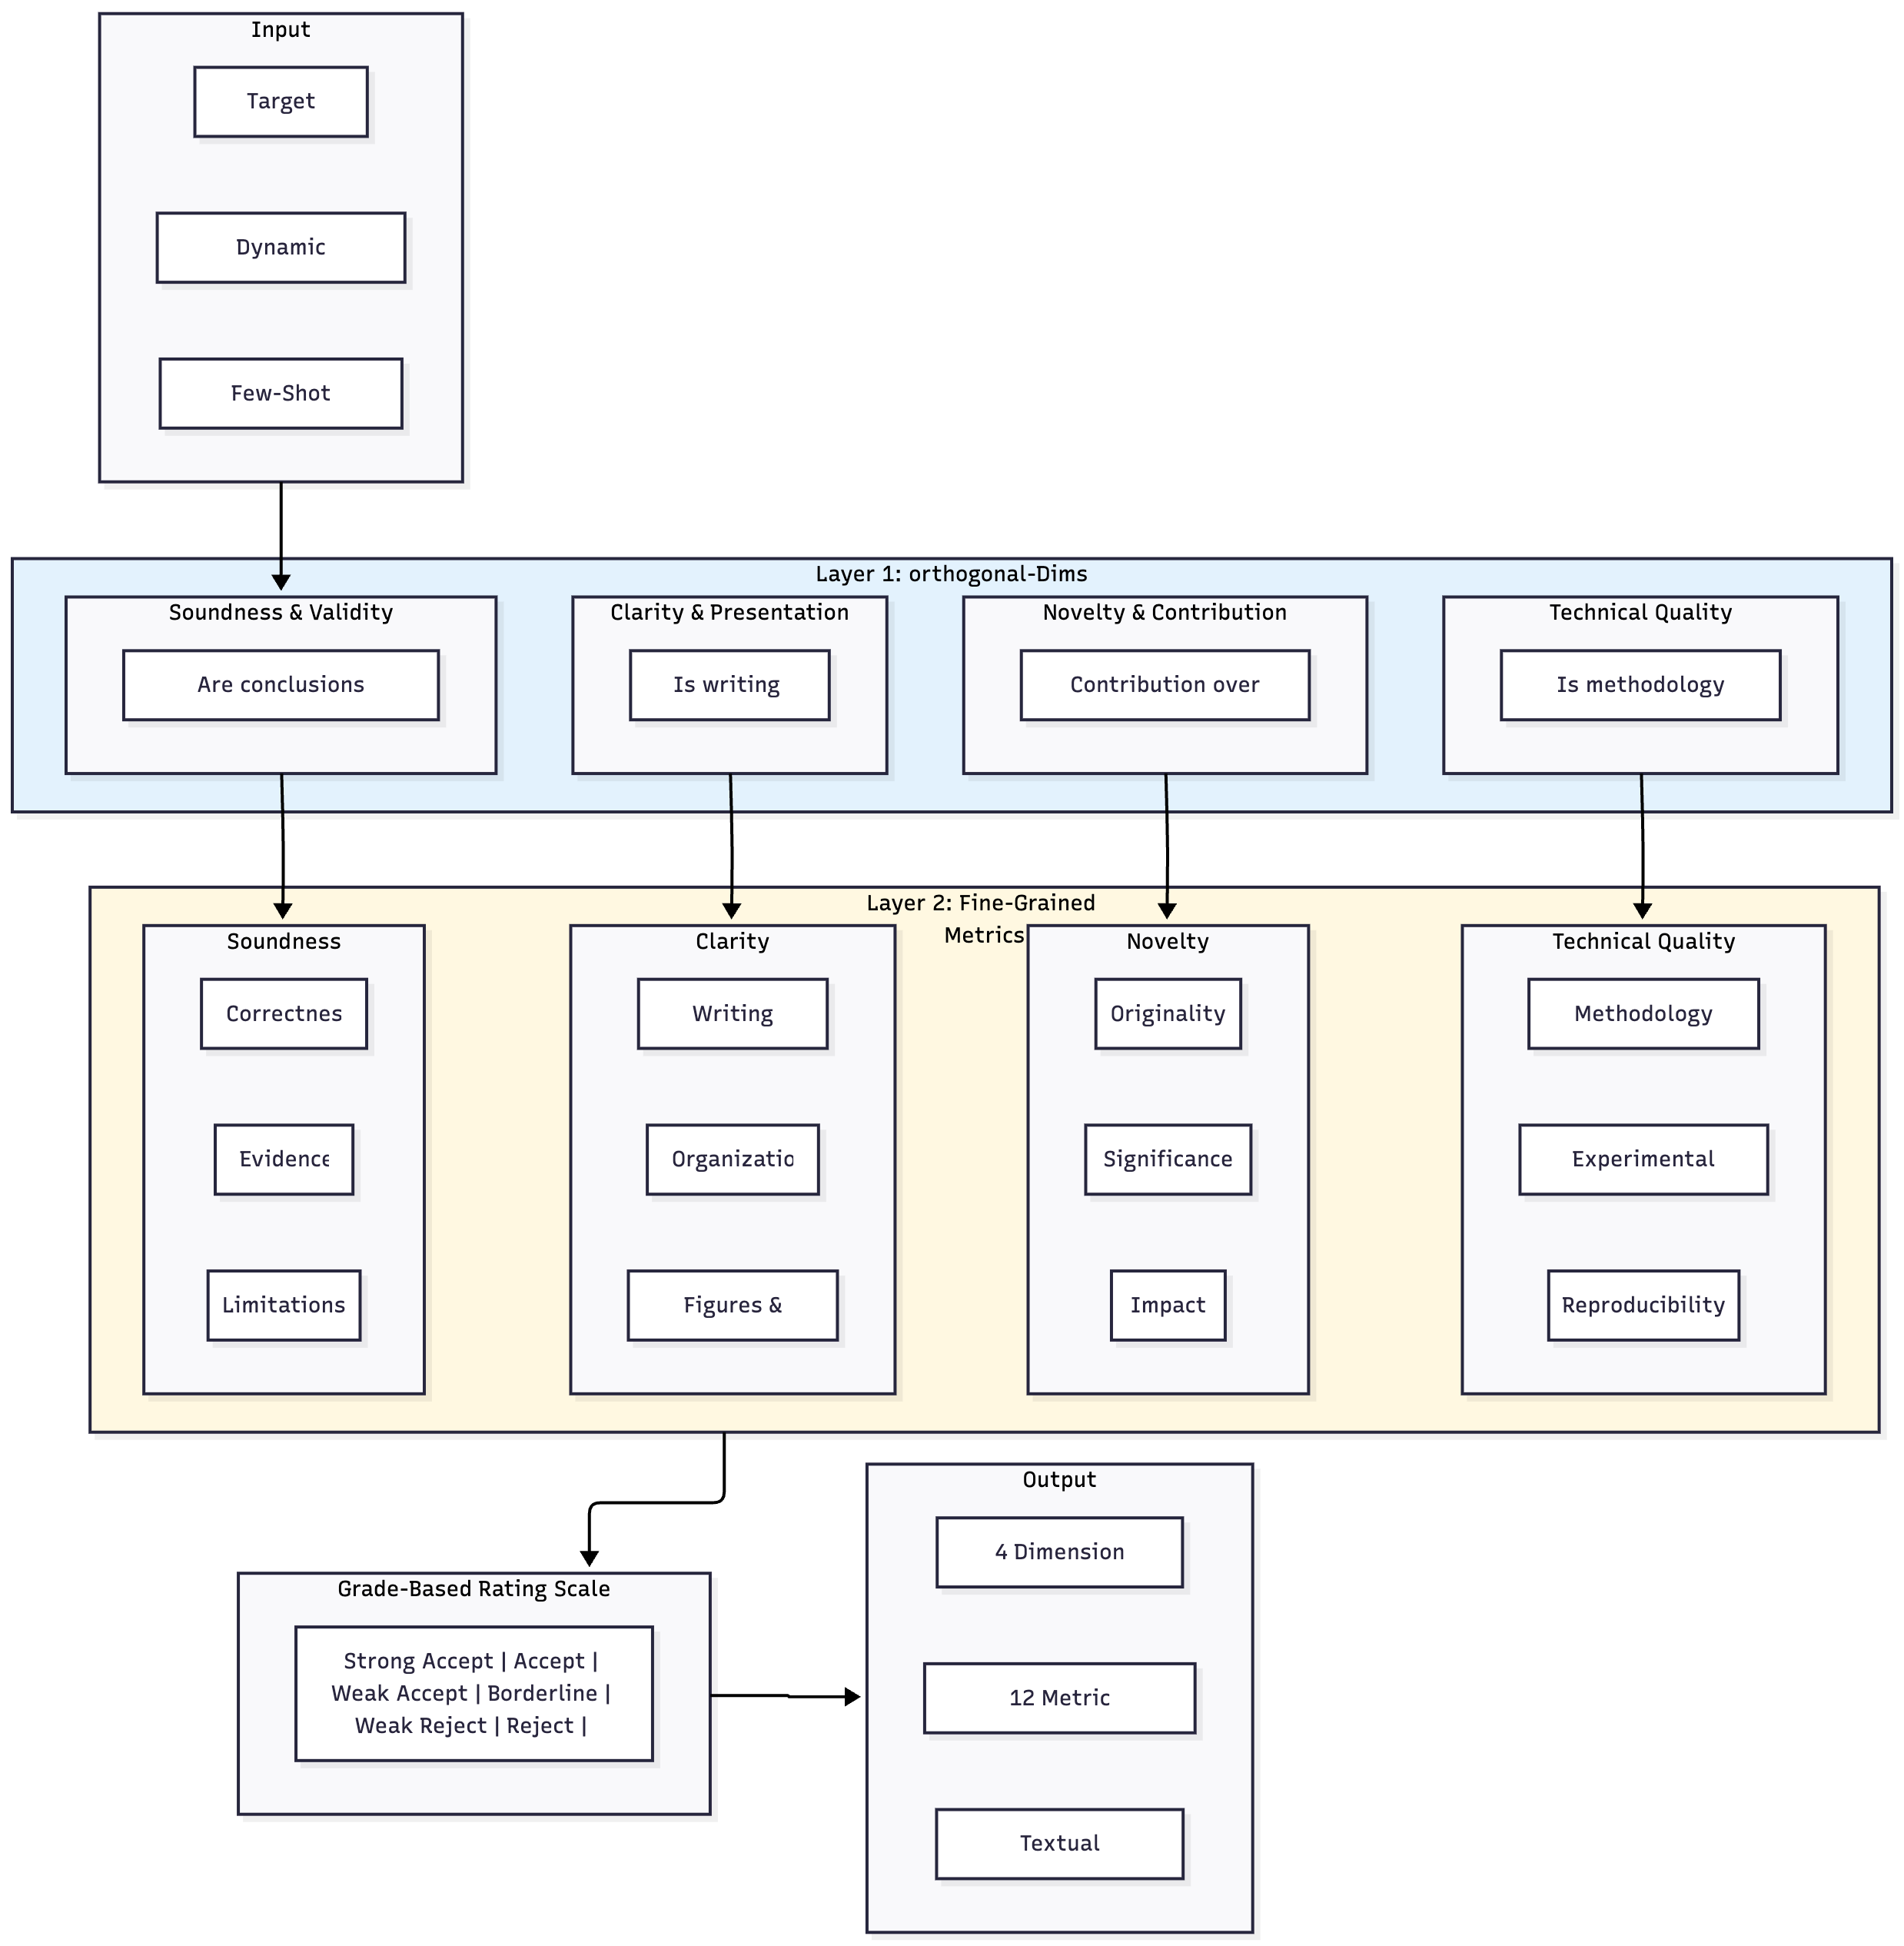
\includegraphics[width=\linewidth]{figures/evaluation_dims.png}
    \caption{Phase 3: Two-Layer Evaluation Structure. Layer 1 defines four orthogonal dimensions; Layer 2 provides 12 fine-grained metrics. Each dimension is evaluated independently using grade-based ratings.}
    \label{fig:evaluation_dims}
\end{figure}

\paragraph{Layer 1: Four Orthogonal Dimensions.} Each dimension evaluates one aspect independently:

\begin{itemize}[nosep,leftmargin=*]
    \item \textbf{Technical Quality}: Is the methodology correct and rigorous? (Ignores novelty and presentation)
    \item \textbf{Novelty \& Contribution}: What is the incremental contribution over SOTA? (Ignores execution quality)
    \item \textbf{Clarity \& Presentation}: Is the paper clearly written? (Ignores technical correctness)
    \item \textbf{Soundness \& Validity}: Are conclusions adequately supported? (Ignores method complexity)
\end{itemize}

The orthogonality principle ensures a paper can be rated as ``novel but poorly written'' or ``clear but unsound'' without forcing artificial coupling.

\paragraph{Layer 2: Fine-Grained Metrics.} Each dimension decomposes into three specific metrics:

\begin{table}[h]
\centering
\caption{Two-Layer Evaluation Rubric}
\label{tab:rubric}
\small
\begin{tabular}{@{}ll@{}}
\toprule
\textbf{Dimension} & \textbf{Fine-Grained Metrics} \\
\midrule
Technical Quality & Methodology Rigor, Experimental Design, Reproducibility \\
Novelty \& Contribution & Originality, Significance, Potential Impact \\
Clarity \& Presentation & Writing Quality, Organization, Figures \& Tables \\
Soundness \& Validity & Correctness of Claims, Evidence Adequacy, Limitations \\
\bottomrule
\end{tabular}
\end{table}

\subsubsection{Rating Rubric}

\paragraph{Grade-Based Ratings.} A critical design decision is using grades rather than numerical scores. LLMs exhibit numerical instability---repeated runs produce different scores for identical inputs~\cite{zhou2024llm}. Grade-based ratings aligned with conference practices provide stability:

\begin{table}[h]
\centering
\caption{Seven-Point Rating Scale}
\label{tab:rating_scale}
\small
\begin{tabular}{@{}lll@{}}
\toprule
\textbf{Grade} & \textbf{Interpretation} & \textbf{Internal Value} \\
\midrule
Strong Accept & Significantly exceeds standards, major contribution & 10 \\
Accept & Meets top-venue standards, clear contribution & 8 \\
Weak Accept & Acceptable with minor issues & 6 \\
Borderline & At the threshold, needs improvement & 5 \\
Weak Reject & Below standards, notable problems & 4 \\
Reject & Does not meet standards, major revision needed & 3 \\
Strong Reject & Fundamental flaws, unsuitable for publication & 1 \\
\bottomrule
\end{tabular}
\end{table}

Internal numerical values are used only for aggregation and never exposed to the LLM during evaluation.

\subsubsection{Prompt Design}

Our prompts follow a structured five-component format designed to maximize output consistency and quality.

\paragraph{Component 1: Role Definition.} The prompt establishes the LLM as ``HorizonBench Reviewer,'' an expert academic reviewer with interdisciplinary experience, tasked with objective evaluation following established academic norms.

\paragraph{Component 2: Context Injection.} The prompt includes: the Paper Schema from Phase 1, the Dynamic Benchmark from Phase 2, and the four-dimension evaluation rubric. This grounds evaluation in paper-specific context.

\paragraph{Component 3: Few-Shot Examples.} We include 2--4 real reviews from OpenReview, strategically sampled:
\begin{itemize}[nosep,leftmargin=*]
    \item 1--2 accepted examples (Strong Accept, Accept) demonstrating positive evaluation
    \item 1--2 rejected examples showing critical assessment and rejection rationale
\end{itemize}
This balanced sampling teaches the model to recognize acceptance boundaries.

\paragraph{Component 4: Task Decomposition.} Following chain-of-thought principles~\cite{wei2022chain}, we decompose evaluation into explicit stages: (1) \textbf{Comprehension}: summarize paper's aim, method, and findings; (2) \textbf{Analysis}: assess each dimension with specific evidence; (3) \textbf{Synthesis}: prioritize strengths, weaknesses, and actionable recommendations.

\paragraph{Component 5: Output Format.} We enforce JSON output schema for structured parsing:

\begin{verbatim}
{
  "dimensions": {
    "technical_quality": {"grade": "Accept", "justification": "..."},
    "novelty": {"grade": "Strong Accept", "justification": "..."},
    ...
  },
  "overall_rating": "Accept",
  "confidence": "High",
  "strengths": ["...", "..."],
  "weaknesses": ["...", "..."],
  "suggestions": ["...", "..."]
}
\end{verbatim}

% -------------------------------------------------
\subsection{Output and User Interface}
% -------------------------------------------------

The final output is a comprehensive evaluation report designed for multiple stakeholders. Figure~\ref{fig:output_report} shows the report structure.

\begin{figure}[t]
    \centering
    \includegraphics[width=0.9\linewidth]{figures/output_report.png}
    \caption{Output Report Structure. The report provides hierarchical information from overall rating through dimension scores, benchmark context, reviewer summary, meta-review synthesis, and actionable feedback.}
    \label{fig:output_report}
\end{figure}

\paragraph{Report Components.} The structured report contains six sections:

\begin{enumerate}[nosep,leftmargin=*]
    \item \textbf{Header}: Paper metadata, overall rating, and confidence level
    \item \textbf{Dimension Scores}: Four dimension grades with brief justifications
    \item \textbf{Benchmark Context}: Number of related papers found, current SOTA, paper positioning
    \item \textbf{Reviewer Summary}: Individual ratings from GPT, Claude, and DeepSeek
    \item \textbf{Meta Review}: Consensus points, divergence resolution, decision rationale
    \item \textbf{Feedback}: Itemized strengths, weaknesses, and improvement suggestions
\end{enumerate}

\paragraph{Output Formats.} The system supports multiple export formats: JSON for programmatic processing and integration, PDF for archival and formal review records, and interactive web dashboard for exploratory analysis.

\paragraph{Use Cases.} The design serves three primary stakeholders: (1) \textbf{Conference Organizers}: desk-reject triage and reviewer assignment assistance; (2) \textbf{Reviewers}: preliminary analysis reducing cognitive load; (3) \textbf{Authors}: pre-submission feedback identifying improvement areas before formal submission.
